\chapter{Road Pricing}
\label{ch:roadpricing}
% ##################################################################################################################

\hfill \textbf{Author:} Kai Nagel

\begin{center} 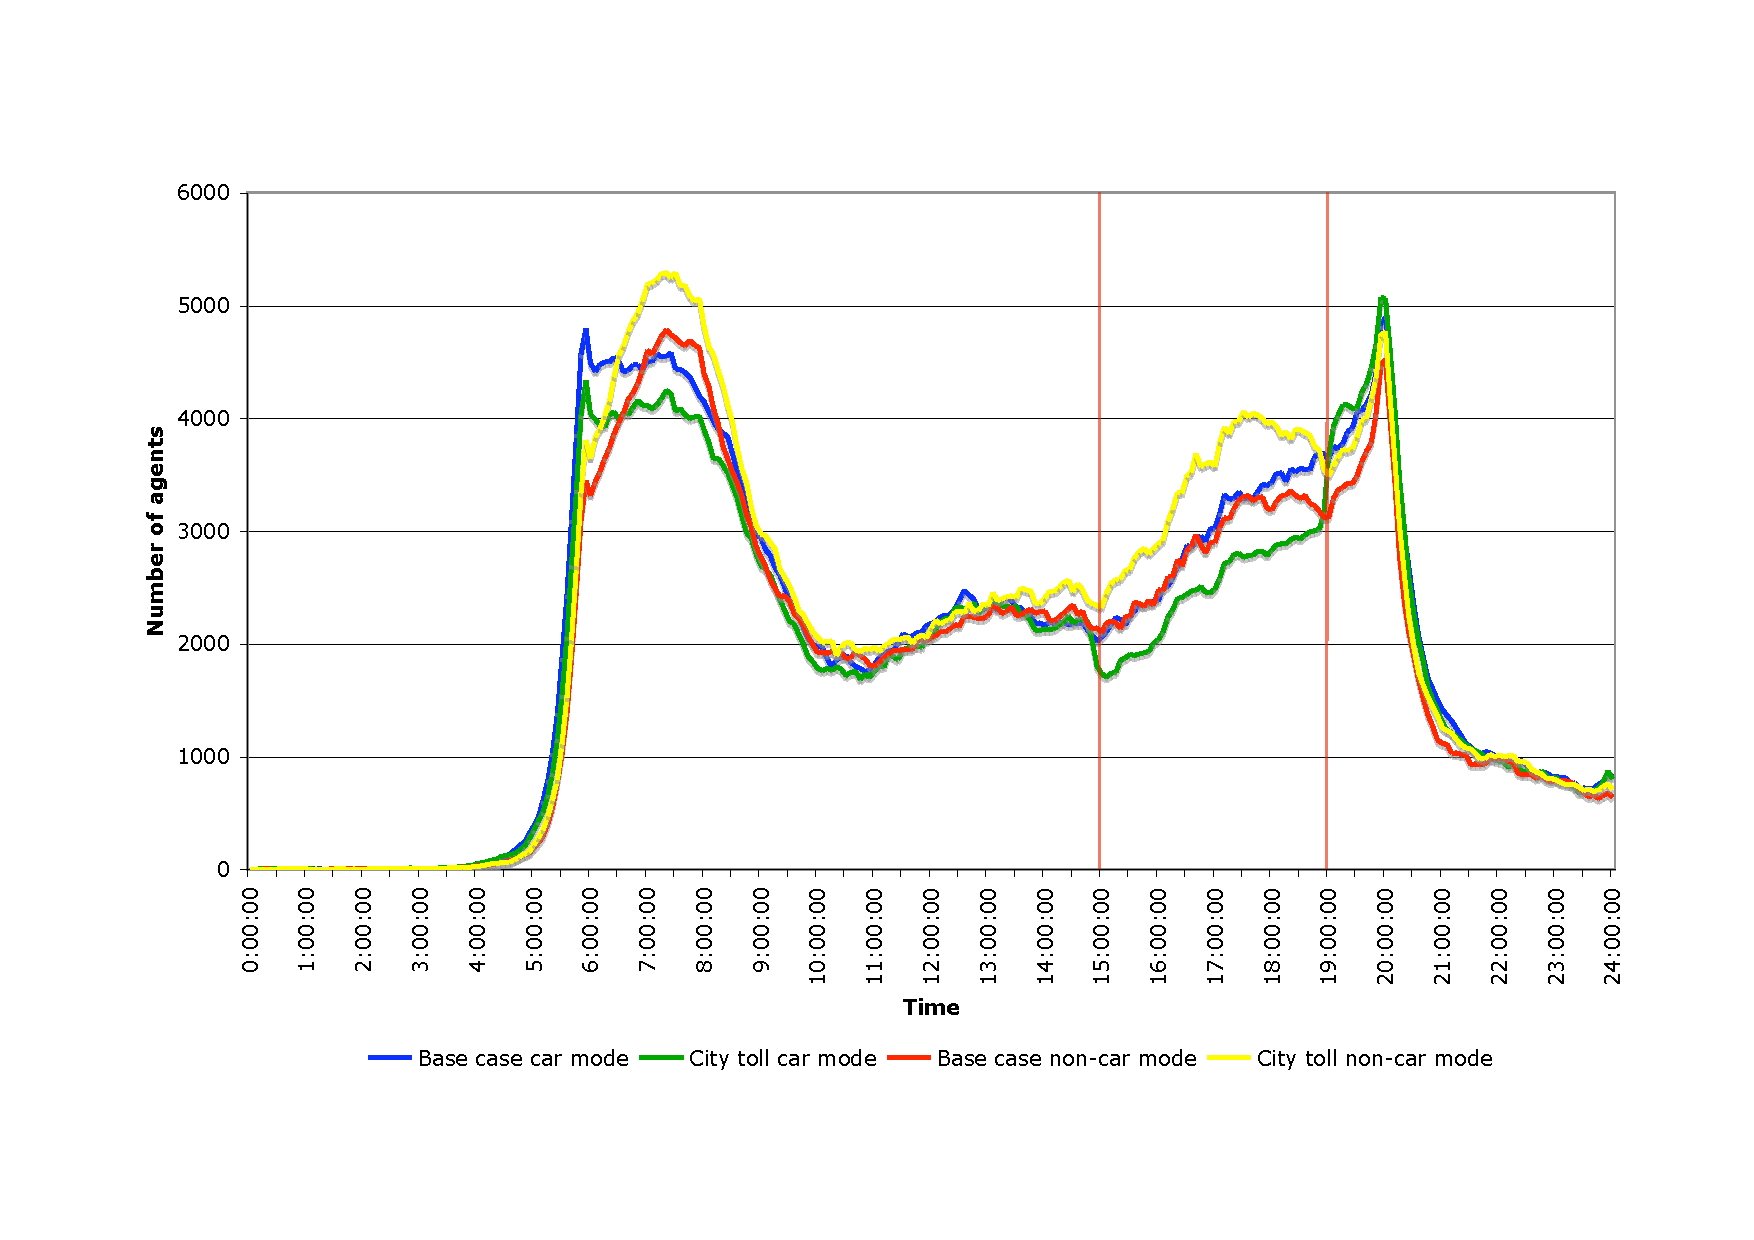
\includegraphics[width=0.6\textwidth, angle=0]{extending/figures/roadpricing/583vs585onRoute.pdf} \end{center}

\editdone{This text has undergone the professional edit. Please no grammatical changes anymore! They are most-probably wrong.}

\createStandardInformation{roadpricing}{\lstinline{RunRoadPricingExample} class}{roadpricing}%
{\citet{RieserBeuckNagel2007early-toll-zrh-etc,RieserEtAl2008ITMEveningToll,GretherEtAl2008ERSARoadPricing}}

\kaitodo{check copyrights}

% ##################################################################################################################
\section{Introduction}
\label{sec:roadpricing-intro}
Roadpricing is a controversial policy measure \citep[e.g.,][]{ButtonVerhoef_1998}. Its implementation in \gls{matsim} is conceptually straightforward \citep{%
%
RieserBeuckNagel2007early-toll-zrh-etc,RieserEtAl2008ITMEveningToll,GretherEtAl2008ERSARoadPricing
%
}: Essentially, for each vehicle entering a link at a given time, the appropriate toll is computed and charged to the vehicle's driver. The scoring function will pick this up by the term (see Equation~(\ref{eq:tdisutility}))
\[
S_{trav,car,q} = ... + \beta_{m} \cdot (\tau) + ... \ ,
\]
where $\tau$ is change in the monetary budget invoked by all toll payments (usually negative) and $\beta_{m}$ is the marginal utility of money (also see Chapter~\ref{ch:scoring} and Chapter~\ref{ch:economicEval}). The driver then takes this into account making decisions, \eg  for route choice, departure time choice, mode choice, destination choice, etc., and then trades off toll payments with other elements of his or her scoring function.

It should be clear that this automatically picks up all kinds of heterogeneities, for example:
\begin{itemize}\styleItemize
\item Traveling at a different time may lead to a different toll, but possibly also to different schedule delay costs (Section~\ref{sec:schedule-delay-costs}). 
\item Different vehicle types may be charged different tolls. \citep{KickhoeferNagel2013EmissionInternalizationNETS}.
\item Different travelers may have different time values, \citep{NagelKickhoeferJoubert2014HeterogeneousVoTsPROCEDIA}, which may even vary according to the time of day.
\end{itemize}

However, one challenge is that the innovative modules (Section~\ref{sec:strategymodules}) must be consistent with the scoring now modified by road pricing. The approach just described will not work if, for example, the router consistently generates toll-avoiding routes for a synthetic person with a high time value,  who would normally wish to pay for a faster option. In a case like this, if a suitable route is never generated, the scoring cannot identify it, giving  the choice process no chance to select it in subsequent iterations.

However, processing every detail for each individual, \ie not only the marginal utility of money, but also specific time pressure at the route search time, is quite complex.
%% , in particular since time pressure is only implicitly given by the first derivative of the scoring function \emph{given the agent's current schedule}.  

An alternative approach is to make the router \emph{randomizing}, \ie to run it with a randomly generated time value every time necessary for a given person. Computational experiments with this approach produce solutions for synthetic travelers approximately as good, or even better, than an ``engineered'' router \citep{NagelKickhoeferJoubert2014HeterogeneousVoTsPROCEDIA}. At the same time, the software consistency burden is significantly reduced, noticeable in the smaller amount of information to be extracted from the agent during each router call.

% ##################################################################################################################
\section{Some Results}
\subsection{Effect of an Afternoon Toll on Morning Traffic}
In a first demonstration of capabilities, an afternoon toll for the Zürich area was simulated. While this is an unlikely policy scheme, it still clearly demonstrated the advantage of the integrated approach over other approaches. Not only did the synthetic travelers switch to public transit, but they also did so for the morning rush hour, where no toll was charged (Figure~\ref{fig:afternoon-toll}). Thus, the \gls{matsim} approach proved its ability to affect the whole daily plan, not just the trip. For more information, see \citet{RieserEtAl2008ITMEveningToll}.
%
% ------------
\createfigure%
{An afternoon city toll (between 3\,pm and 7\,pm) affects mode choice not just during the toll time, but also in the morning}%
{An afternoon city toll (between 3\,pm and 7\,pm) affects mode choice not just during the toll time, but also in the morning}%
{\label{fig:afternoon-toll}}%
{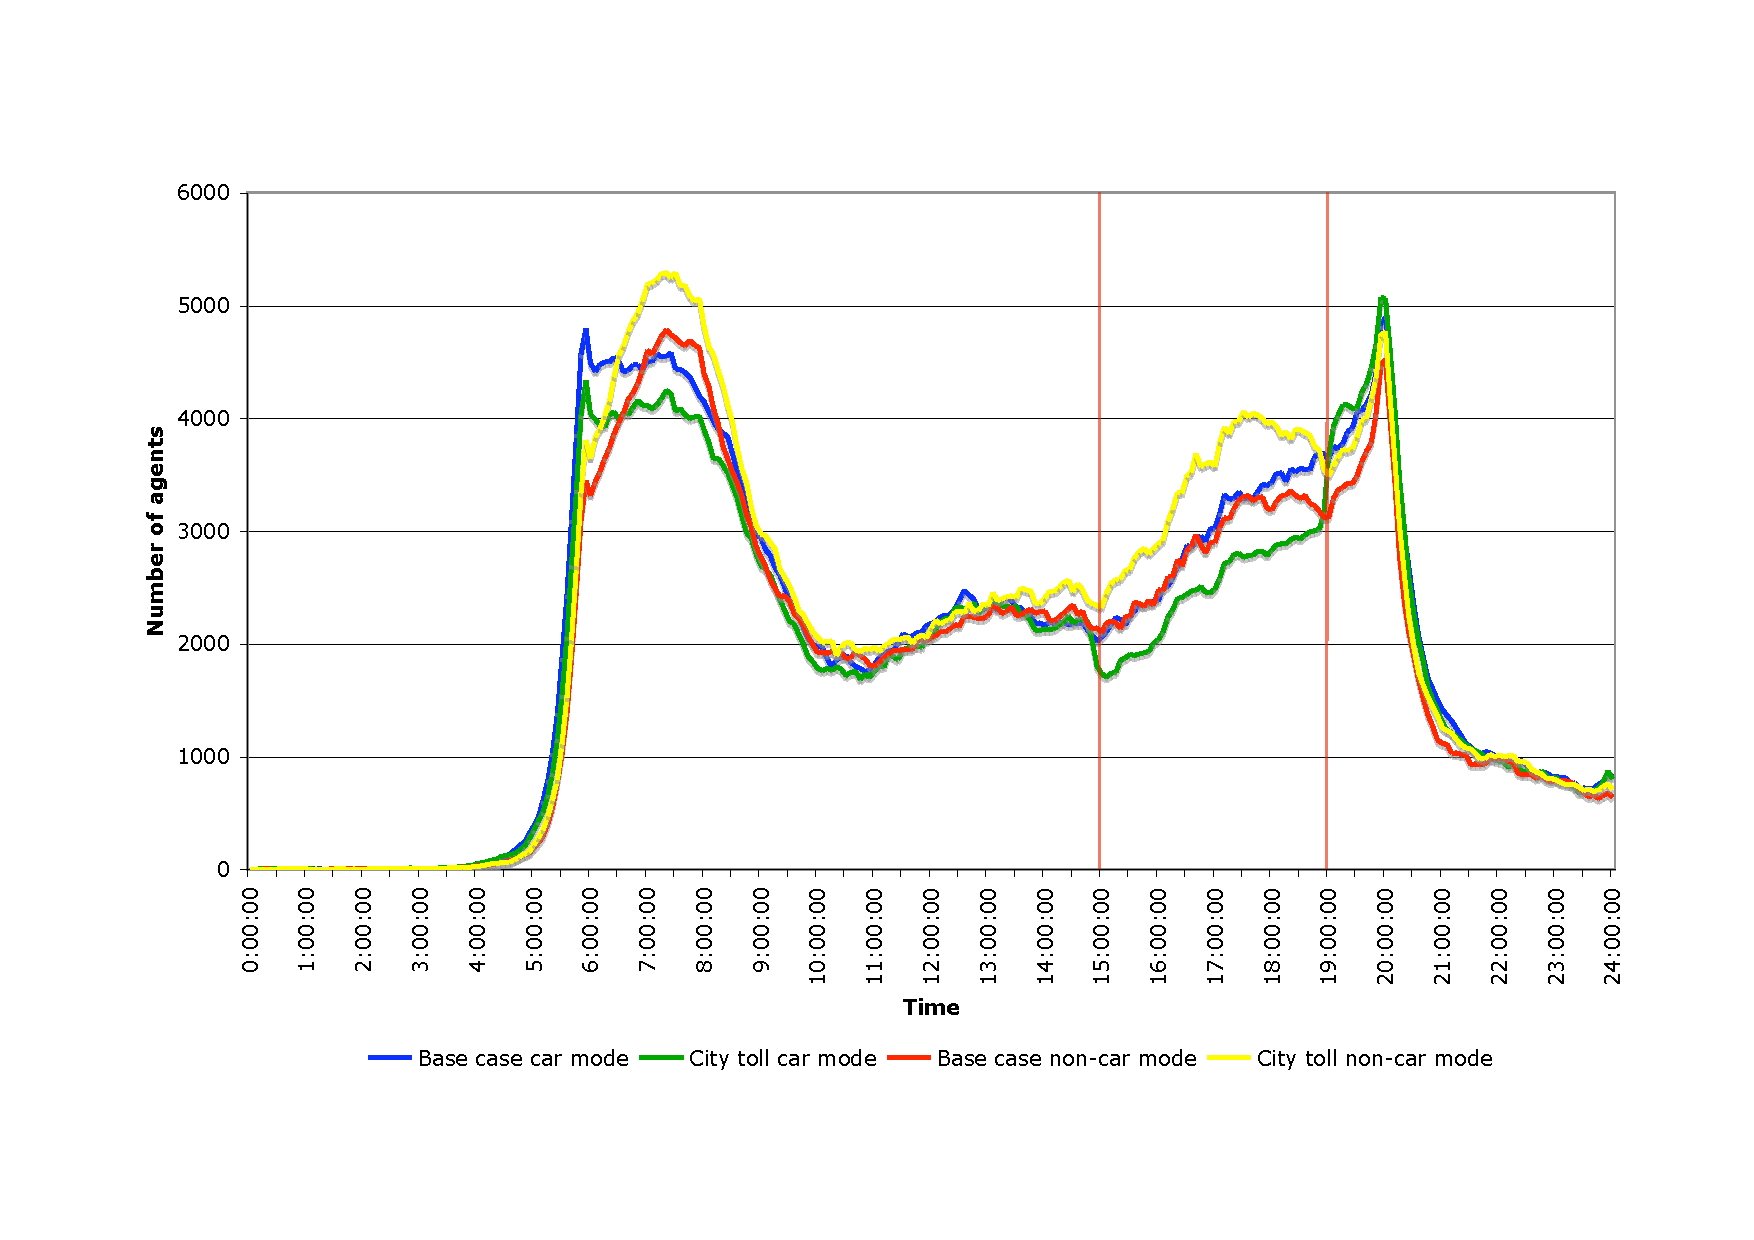
\includegraphics[width=0.99\hsize,trim=2cm 2.5cm 2cm 3cm,clip]{extending/figures/roadpricing/583vs585onRoute.pdf}}%
{}
% ------------
%% \benjamin{Es gibt ein ähnliches Bild auch in meiner Diss...Verweis siehe unten.}
%% \benjamin{One could also cite NagelGretherEtc2008ag-based-evaluation...}

% ============================================================================
\subsection{Income-Dependent Values of Time}
Similar to \citet{RieserEtAl2008ITMEveningToll}, \citet{KickhoeferEtAl2010EconomicEvaluationPublicAcceptanceRoadPricingKuhmo, Kickhoefer_PhDThesis_2014} introduced a distance-based morning peak toll on the same links between 6:30\,am and 9\,am. Toll levels were incrementally increased from 0.28\,$CHF/km$ up to an almost prohibitive price of 44.80\,$CHF/km$. The studies assume income-dependent utility functions with a decreasing marginal utility of money. The goal was to (i) identify the welfare-maximizing \citep[see e.g.,][Section~2.5]{TirachiniHensherRose_TransResB_2014}
% \karen{"welfare" has a very marked connotation in US English. To what do we refer? Social good or fairness? Feeling of financial well-being? Financial comfort/pain level? Let's try to reword. See also line 65-66.} 
toll level, which is potentially dependent on the aggregation rule of user benefits (see Chapter~\ref{ch:economicEval}), and (ii) to investigate distributional aspects of such pricing schemes.
%
The studies showed that changes in travel patterns resulting from the morning peak toll impacted the whole day, affecting traffic patterns in the afternoon.
%
Furthermore, the study showed that such a parametric approach is capable of identifying the welfare-maximizing toll level. However, results also indicated that the overall welfare effect level depends strongly on the aggregation rule for user benefits, \ie if one first monetizes individual utilities and then adds up, or first adds up utilities and then monetizes. 
Even the sign of that effect might not be stable depending on that choice.
%
For more information, please refer to the two studies above.

%% \kai{todo}
%% \benjamin{done?}

% ============================================================================
\subsection{Integrated Passenger and Freight Toll Simulation for the Gauteng Province in South Africa}
A large scale application was undertaken for the Gauteng province in South Africa (Chapter~\ref{ch:gauteng}). It is based on the so-called e-toll, which was switched on in December~2013. The e-toll should, logically, charge different rates for different vehicle types, with higher rates for heavy trucks. Again, logically, this should go along with higher time values of the driver-vehicle-units.  Somewhat surprisingly, this turned out to be difficult to do with the \gls{matsim} software structure in place when the project was started in 2008. While it was easy to charge the freight vehicles a higher toll, it was difficult to give different replanning methods and different scoring function to the freight population; it was essentially impossible to feed the router with different time values for the freight population. This was an important driver for much development in recent years, including making the scoring function more accessible (Section~\ref{sec:scoring-extension-point}), allowing different replanning strategies for different sub-populations (Section~\ref{sec:strategymodules}), and reducing consistency requirements between the router, the vehicle-based toll and the driver-based scoring function \citep{NagelKickhoeferJoubert2014HeterogeneousVoTsPROCEDIA}.

The simulation, as expected, predicts reduced traffic volumes on the tolled roads and increased volumes elsewhere (Figure~\ref{fig:gauteng-toll-volumes}).

% ------------
\createfigure%
{Predicted differences in link volumes after introduction of the toll (red: higher volumes, green: lower volumes)}%
{Predicted differences in link volumes after introduction of the toll (red: higher volumes, green: lower volumes)}%
{\label{fig:gauteng-toll-volumes}}%
{\includegraphics[width=0.8\hsize,trim=0 0 0 0,clip]{extending/figures/roadpricing/abs-diff-link-vol-vot20-24h}}%
{}
% ------------

% ##################################################################################################################
\section{Invocation}
\subsection{Minimal}
A minimum amount of infrastructure is necessary when running roadpricing from the command line. For this, the \gls{matsim} \gls{jar}, its libraries, \emph{and} the roadpricing \gls{jar} need to be downloaded, either from a release or from the nightly builds (Section~\ref{sec:releases-builds}). After unzipping all zip files, the necessary command is (may need slight refactoring with new formats):
\begin{lstlisting}
java -Xmx2000m -cp MATSim.jar:roadpricing-.../roadpricing-
   ...jar org.matsim.roadpricing.run.RunRoadPricingExample config.xml  
\end{lstlisting}
where \lstinline$config.xml$ needs to contain a section
\begin{xml}
<module name="roadpricing" >
...<param name="tollLinksFile" value="<path>/<tollfilename>" />
</module>
\end{xml}
The toll file looks like this:
%
\begin{xml}
<roadpricing type="link" name="abc">
   <links>
      <link id="11">
         <cost start_time="05:00" end_time="10:00" amount="1." />
         <cost start_time="17:00" end_time="20:00" amount="1." />
      </link>             
      <link id="12" />
   </links>

   <!--this is for all links with no cost entry above:-->
   <cost start_time="05:00" end_time="10:00" amount="2.00"/>

</roadpricing>
\end{xml}
%
As one can see, there is a section where each link can be entered separately. A separate cost structure for each link is also possible. All links that are listed without a cost structure employ the general cost structure listed at the end. Links not listed are without toll.

% ============================================================================
\subsection{Toll Schemes}
\paragraph{Link toll} The example refers to the ``link'' toll scheme, indicated by \lstinline$type="link"$. It charges the amount specified on the link.

\paragraph{Distance toll} Another useful scheme is ``distance'', indicated by \lstinline$type="distance"$. Here, the \lstinline$amount$ is interpreted as amount per length unit (see Section~\ref{sec:unitsconventions}). This is most useful, with only a list of tolled links and a uniform distance cost for all these links noted at the end of the file.

\paragraph{Area toll} The simulation of an \emph{area toll}---\ie a toll where one has to pay a flat fee for a given time period, often a day, once one drives anywhere inside the area---suffers from a combinatorial challenge: driving through the tolled area early in the day may only pay off if one can re-use the permit later in the day. The code, in principle, addresses that by routing the agent twice: once under the assumption of a zero toll and once under the assumption of a very large toll. Afterward, the toll is added to the generalized cost of the first option, then both options are compared.  
%
In the end, the approach suffered from the same consistency burden as the general approach (see end of Section~\ref{sec:roadpricing-intro}): the router made the decision about the better variant, rather than leaving the decision to the agent. It should be re-implemented using the same principles as \citet{NagelKickhoeferJoubert2014HeterogeneousVoTsPROCEDIA}.

\paragraph{Cordon toll} The cordon toll scheme was derived from the area scheme; one could use the same file, listing all area links, for the cordon toll as well. The code ensured that toll was only charged when a vehicle moved from an untolled link to a tolled link---thereby effectively crossing the cordon. One difficulty with this approach: confusion ensues if there is no connected area and several links in sequence are tolled instead.  Then, if these links are connected, the toll is only charged on the first of them; if there is a small section missing, perhaps overlooked, the toll is charged again. 

% ============================================================================
%\subsection{Invocation as "Script in Java"}

%See Sec.~\ref{sec:roadpricing-stdInfo} under "Invoking the module".

%% The above \lstinline$org.matsim.roadpricing.run.Main$ class can also be used as a starting point for one's own ``script in Java'':
%% \begin{lstlisting}
%% public static void main(String[] args) {
%% 	// load the config, telling it to "materialize" the road pricing section:
%% 	Config config = ConfigUtils.loadConfig(args[0], new RoadPricingConfigGroup());
	
%% 	// load the scenario:
%% 	Scenario scenario = ScenarioUtils.loadScenario(config) ;

%% 	// instantiate the controler:
%% 	Controler controler = new Controler(scenario) ;

%% 	// instantiate road pricing and add it as controler listener:
%% 	RoadPricing roadPricing = new RoadPricing() ;
%% 	controler.addControlerListener( roadPricing ) ;

%% 	// run the controler:
%% 	controler.run() ;
%% }
%% \end{lstlisting}

% ##################################################################################################################
%\section{More information}

%See Sec.~\ref{sec:roadpricing-stdInfo}.

%% \url{http://ci.matsim.org:8080/job/MATSim_contrib_M2/org.matsim.contrib$roadpricing/javadoc/?}

% ##################################################################################################################
% Local Variables:
% mode: latex
% mode: reftex
% mode: visual-line
% TeX-master: "../../main"
% comment-padding: 1
% fill-column: 9999
% End: 
